\chapter{Physical Unclonable Functions}
\label{sec:PUF}

\begin{boxH}
  \textbf{Physical Unclonable Functions} (PUFs) have been introduced as the hardware equivalent of a
  one-way function.
\end{boxH}

Some examples of them are:
\begin{itemize}
  \item things that add some delay on some networks, like Ring Oscillators PUF and Arbiter PUF
  \item the content of the SRAMs at boot time
  \item the re
\end{itemize}
Ideally, it is a cryptographically secure one-way function that generates a digital output
(response) for a given input (challenge) without revealing any predictable mapping between the
challenge and response.

A PUF \textbf{must be}:
\begin{itemize}
  \item computable: its easy to evaluate $y==PUF(x)$
  \item unique: the puf contains some information about the identity of the physical entity
    embedding the PUF
  \item reproducible: $y\approx PUF(x)$ up to a small error
  \item unclonable: given PUF, it is hard to construct a procedure PUF’ such that $PUF(x) \approx
    PUF’(x)$
  \item unpredictable: given a set of CRPs, it is hard to predict $y \approx PUF(x)$
  \item one-way: it is hard to invert the function, even with some errors
\end{itemize}

\begin{section}{PUF Classification}
There are actually different kinds of PUFs, distinguished by their architecture, like silicon and
non-silicon PUFs, or by the size of the challenge-response pairs (CRPs), like strong and weak PUFs.
\begin{figure}[h]
  \centering
  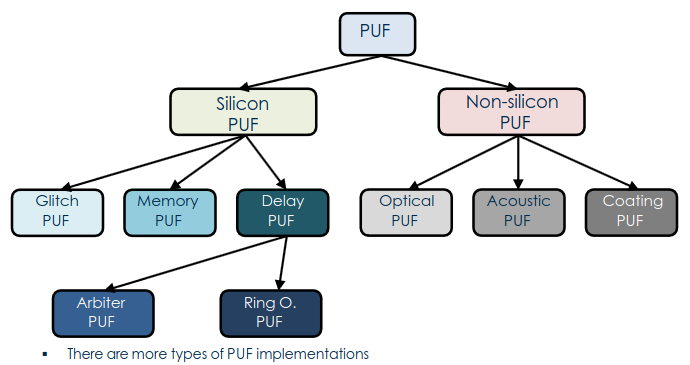
\includegraphics[width=0.5\textwidth]{img/hardware/puf classif.png}
  \caption{Puf Classification}
\end{figure}

\begin{subsection}{PUF architectures}
  \begin{subsubsection}{Ring Oscillator(RO) PUF}
    An RO-PUF is generally composed of N identical ring oscillators (ROs), two multiplexers, two
    counters, and one comparator.\\
    Ideally, ring oscillators should have all the same frequency, but in practice, each one 
    oscillates at a slightly different frequency due to process variations.
    \begin{figure}[h]
      \centering
      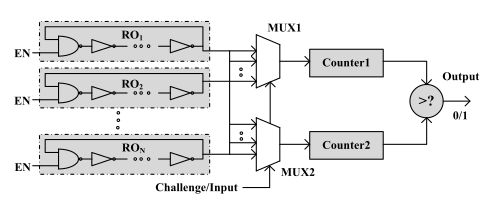
\includegraphics[width=0.5\textwidth]{img/hardware/RO PUF.png}
      \caption{Ring Oscillator PUF}
    \end{figure}
    A challenge is applied to select one pair of ROs, and the number of oscillations of each of the
    ROs in the selected pair is counted and compared to generate bit, based on which
    oscillator from the selected RO pair is faster.\\
    This implementation means that for every set of $N$ ROs, there are $\frac{N(N-1)}{2}$ possible
    pairs, meaning that the entropy of the PUF is $log_2(N!)$.
  \end{subsubsection}
  \begin{subsubsection}{Arbiter PUF}
    Arbiter-PUF is one of the most notable CMOS logic-based PUF architecture that exploits the
    randomness of path delay due to uncontrollable process variation
    \begin{figure}[h]
      \centering
      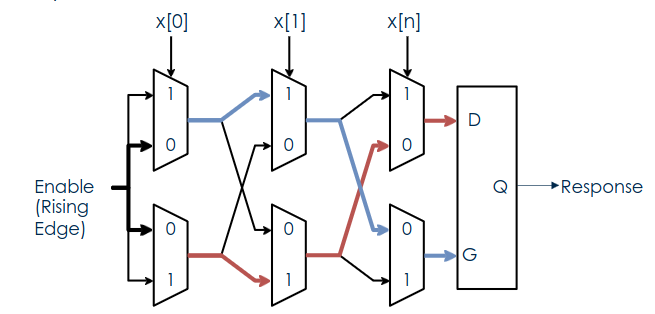
\includegraphics[width=0.5\textwidth]{img/hardware/arbiter puf.png}
      \caption{Arbiter PUF}
    \end{figure}
    Given a pulse at the input of a delay stage, it can traverse through two design-wise identical,
    but different paths (selected by challenge) and reach the final arbiter component. If the signal
    in the upper path reaches the arbiter first, it generates \textit{1} (and vice versa).
  \end{subsubsection}
  \begin{subsubsection}{SRAM-PUF}
    a static random-access memory (SRAM)-based PUF utilizes the widely available SRAM-matrix used
    for many applications in digital systems.\\
    Typically, one SRAM bit is implemented by a symmetrically designed 6-transistor cell, as shown
    in figure \ref{fig:sram_puf}.
    \begin{figure}[h]
      \centering
      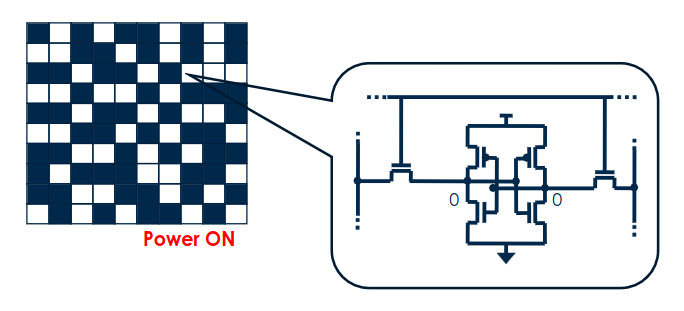
\includegraphics[width=0.5\textwidth]{img/hardware/sram puf.png}
      \caption{SRAM PUF}
      \label{fig:sram_puf}
    \end{figure}
    during the startup in absence of any “write”/programming command, both the logic nodes tend to
    pull up to high voltage. However, only one wins via racing condition to reach high voltage
    (logic 1), and automatically pulls the other node down to low voltage (logic 0). This
    initialization typically depends on the minute process-induced strength mismatch among the cell
    transistors, and is completely unpredictable to an external observer.\\
    The start-up outcome, being strongly tied to the physical process variation, is static and tends
    to produce the same outcome for a given cell over multiple power-ups. Therefore, the startup of
    the SRAM cell can be utilized as a weak PUF for device-intrinsic fingerprint generation.
  \end{subsubsection}
\end{subsection}
\begin{subsection}{Weak and Strong PUFs}
  \begin{paragraph}{Challenge-Response Pair (CRP)}
    A PUF is characterized by a set of challenge-response pairs (CRPs), where the challenge is the
    input to the PUF and the response is the output.\\
    At first, the result of a PUF for a challenge is stored in a database, and when a challenge has
    to be verified, the PUF is re-evaluated and the result is compared to the one in the database.
  \end{paragraph}
  Based on the underlying challenge-response pair (CRP)-space, PUFs can be broadly categorized into
  \textbf{weak} and \textbf{strong} PUFs.\\
  A weak PUF, also known as a physically obfuscated key (POK), typically can be interrogated with a
  very limited number of challenges. Therefore, its CRP-space is extremely small, often even only
  one. Such a PUF can be used for generating cryptographic keys or to identify devices. An SRAM-PUF
  is a notable example of this type.\\
  In contrast, a strong PUF can accommodate a very large number of challenges to produce
  corresponding responses. Ideally, the CRP-space grows exponentially with the length of challenge
  itself. This allows the PUF to undergo multiple queries and use a new challenge-set every time to
  avoid any collision or replay attacks. The arbiter-PUF and ring-oscillator PUF are prominent
  examples of strong PUFs, and can be used for device authentication.
  \begin{figure}
    \centering
    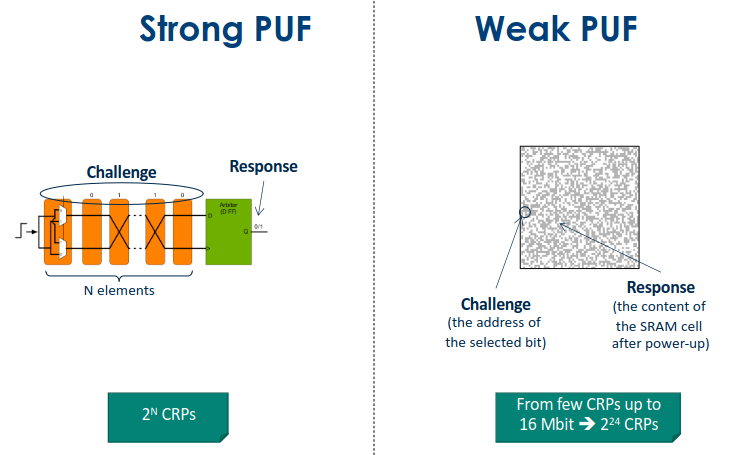
\includegraphics[width=0.5\textwidth]{img/hardware/w-s puf.png}
    \caption{Weak and Strong PUFs}
  \end{figure}
\end{subsection}
\end{section}

\begin{section}{Attacks on PUF}
  There are several attacks on PUFs, like:
  \begin{itemize}
    \item \textbf{Exhaustive Reading} of a weak PUF: Reading out the only 1 CRP on memory PUFs
      On-chip channel
    \item \textbf{Modeling Attacks} on a strong puf: Constructing a model of the PUF to predict the
      response
    \item \textbf{Side-Channel Attacks} analysis: read the leaked data from the PUF
  \end{itemize}
\end{section}
\begin{section}{Restricting Access to PUF}
  An attacker could carry out a MITM attack to intercept the challenge and response. To prevent
  this, the response of the PUF should be made indeterminable to the attacker.\\
  To do so, a shared secret with the PUF is necessary, and to do so, the responses are combined
  with hash values. Its also possible to protect the challenge in the same fashion.
\end{section}
